\section{연구 결과}

\subsection{후드 제작}


본 연구에서는 연구 과정에서 제시한 부품들을 3D프린터로 출력 후 조립하여 Fig.\ref{cover}와 같이 이를 천체망원경의 후드처럼 부착시키는 것에 성공하였다. 앞서 소개하였듯, 후드의 지름은 망원경에 따라 달라질 수 있으므로 다른 망원경에 대한 후드를 제작할 때에는 이에 맞추어 새로 제작하여야 한다.
 
\begin{figure}[h]
	\begin{center}
		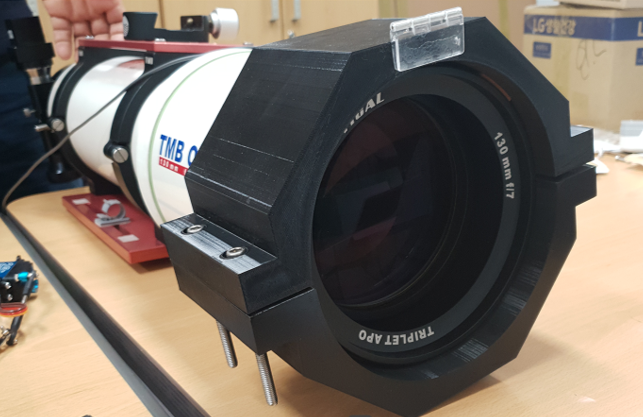
\includegraphics[width = 8cm]{cover}
	\end{center}
\caption{제작한 덮개를 천체망원경에 씌운 모습}
\label{cover}
\end{figure}

경첩은 처음에는 사진에서 사용된 것처럼 플라스틱 소재를 사용하였지만, 이후 금속 소재로 대체하였다. 플라스틱 소재의 경첩은 내구성에서 문제가 있었으며, 3D프린터로 출력한 부품과 접착하기 위해서 여러가지 조건이 필요했기 때문에 안정적이지 않았다. 반면에 금속으로 제작된 경첩은 가운데 뚫려있는 구멍을 활용하여 후드와 안정적으로 결합할 수 있었으며, 내구성또한 뛰어났기 때문에 원격 제어에 적합한 조건들을 갖추고 있다. Fig. \ref{hinge}와 같이 개선된 힌지는 덮개와 아크릴 바흐티노프 마스크 사이를 납작볼트를 이용하여 연결할 수 있으며, 이는 접착제를 이용하여 붙이는 방법보다 간단하고 오래 사용할 수 있다.

 \begin{figure}[h]
	\begin{center}
		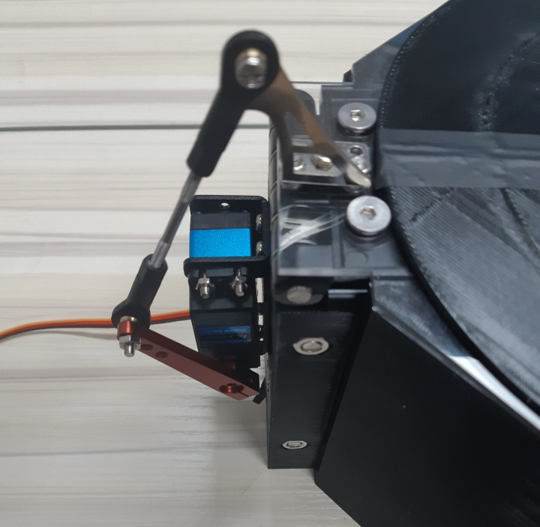
\includegraphics[width = 6cm]{hinge}
	\end{center}
	\caption{개선한 경첩 및 서보모터}
	\label{hinge}
\end{figure}

\subsection{바흐티노프마스크 제작}

Astrojargon을 이용하여 출력한 바흐티노프마스크는 D값을 106, focal length 값을 530으로 출력하였으며, 덮개의 아크릴에 붙이기 편리하도록 지름을 아크릴과 같은 크기로 제작하였다. 출력 과정 중 바흐티노프 사이즈의 크기가 크기 때문에 4조각으로 나누어서 출력하였으며, 빛이 새는 것을 방지하기 위해 나중에 이를 검은 색 테이프로 봉합하였다. 

 
	\begin{figure}[h]
	\begin{center}
		\begin{tikzpicture}
		\node[anchor=south west,inner sep=0] at (0,0) 
		{
			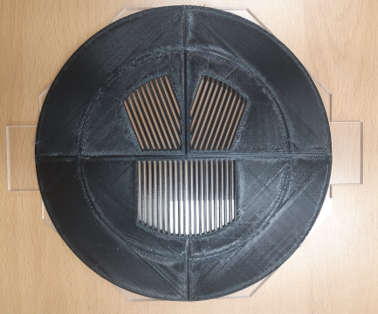
\includegraphics[height=4.5cm]{mask1}
			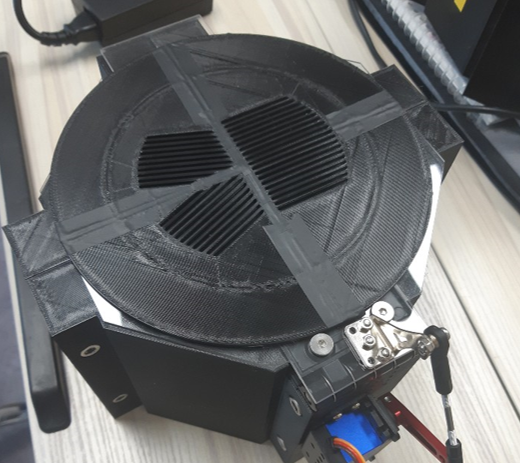
\includegraphics[height=4.5cm]{mask2} 
		};
		\draw (0.3, 4.2) node {(a)};
		\draw (5.9, 4.2) node {(b)};
		\end{tikzpicture}
	\end{center}
	\caption{(a) 4조각으로 나누어서 출력한 FSQ106의 바흐티노프 마스크 (b) 출력된 마스크를 경통에 붙인 모습. 빛이 새지 않도록 접착부를 검은색 테이프로 접합시켜 고정하였다.}
	\label{mask}
	\end{figure}


또한, 3D 프린터의 특성상 한쪽 면은 거친 면, 다른 한쪽 면은 평평한 면을 가지고 있는다. 이 때 거리를 일정하게 하기 위해 평평한 면이 아크릴과 붙는 방향으로 고정시켰다.




\subsection{서보모터 제어}

 서보모터는 후드의 옆면에 부착시켜 제어시킨다. 이 때 정확한 위치에 부착시킬 수 있도록 일정한 간격을 두어 실험을 반복하였으며, Fig. \ref{servo}와 같이 적합한 위치를 찾아 고정시켰다. 

서보모터로 마스크를 정확하게 제어하기 위해서는 마스크가 완전히 덮개에 고정될 수 있어야 하므로 이에 맞는 각도를 계산하여 사용하여야 한다.

\begin{figure}[h]
	\begin{center}
		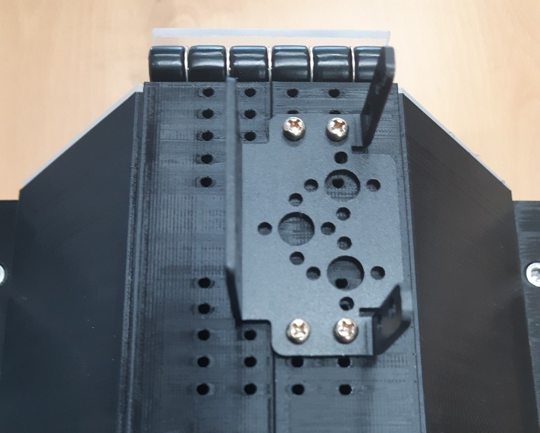
\includegraphics[width = 7cm]{servo3}
	\end{center}
	\caption{후드에 서보모터를 고정하기 위해 볼트를 이용해 고정한 모습}
	\label{servo}
\end{figure}

\subsection{기존 모터포커서 보강}
 제작한 모터포커서는 제어키와 숫자로 이루어져 있는 기호를 통해 통신을 한다. 예를 들어, a에 모터 시계방향 회전을 할당하고 a:100이라는 기호를 입력하면 모터는 시계방향으로 100step만큼 이동하게 되는 것이다. 보강한 모터포커서 또한 이러한 방법을 응용하였으며, 어떤 방법으로 제어에 성공하였는지 서술한다.
 
\subsubsection{열선 제어}

 앞서 설명하였듯 열선의 제어는 전압의 PWM을 이용하여 실행된다. Fig. \ref{PWM}와 같이 시리얼 포트를 통한 입력을 할 때 필요한 기호는 A와 D이며, 0~100의 값을 입력받아 500ms 주기로 값을 변화시킬 수 있도록 설계하였다.
 
  \begin{figure}[h]
 	\begin{center}
 		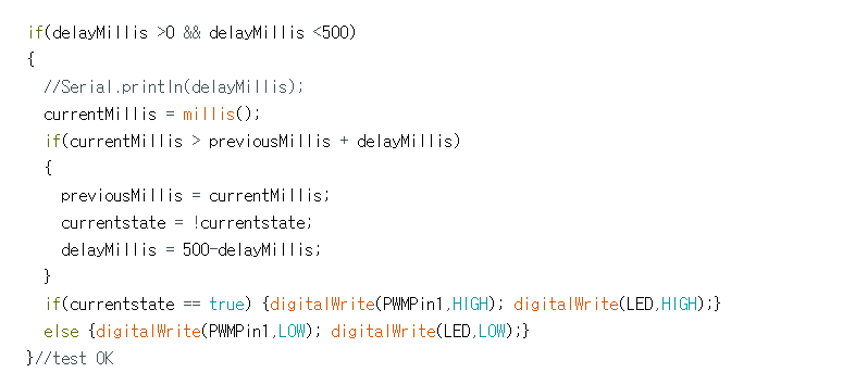
\includegraphics[width = 11cm]{PWMcode}
 	\end{center}
 	\caption{PWM제어를 위한 코드}
 	\label{PWM}
 \end{figure}
 
\subsubsection{EEPROM(Electrically Erasable Read-Only Memory)}

 \begin{figure}[h]
	\begin{center}
		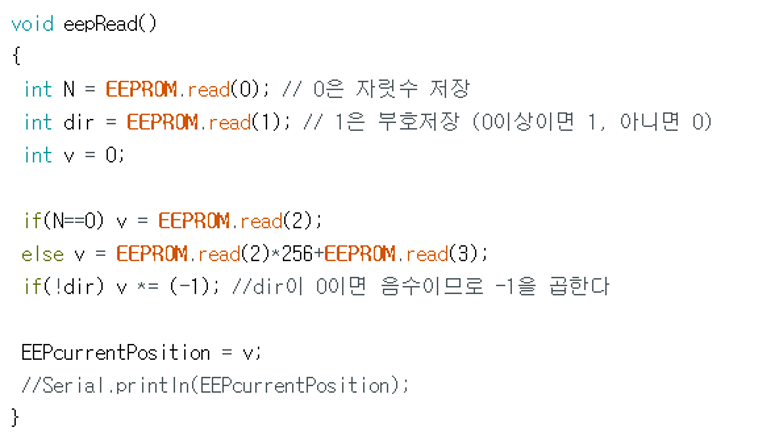
\includegraphics[width = 11cm]{eepread}
	\end{center}
	\caption{EEPROM에서 정보를 읽어오는 과정}
	\label{eepread}
\end{figure}

 모터포커서의 원활한 사용을 위해 저장되어야 하는 값은 모터의 위치를 저장할 수 있는 Position 값이다. Fig.\ref{eepread}은 값을 EEPROM에서 읽어오는 과정을 나타낸 것으로, 모터포커서가 최초로 실행될 때 EEPROM에서 값을 불러오고, 모터를 움직여 값을 변화시킨 직후에 적용된 값을 EEPROM으로 입력시키면 EEPROM값과 모터포커서의 Position 값을 항상 동기화시킬 수 있다.
 
\subsubsection{서보모터 제어}
 일반적인 서보모터 또한 PWM을 응용하여 제어할 수 있으나, 대부분의 라이브러리에서 이미 그 값들을 적용시켜놓은 최적화 함수가 존재한다. 이를 활용하여 서보모터를 원하는 각도로 움직일 수 있도록 펌웨어 상에 코드를 제작하였다. 특히나 OLED를 활용하여 덮개에 부착된 마스크를 정확하게 제어할 수 있도록 하였다.
 
 시리얼 포트를 통한 입력을 할 때 필요한 기호는 N이며, 오직 0과 1만을 입력받아 각각의 상태로 서보모터를 제어한다.

	\begin{figure}[h]
	\begin{center}
		\begin{tikzpicture}
		\node[anchor=south west,inner sep=0] at (0,0) 
		{
			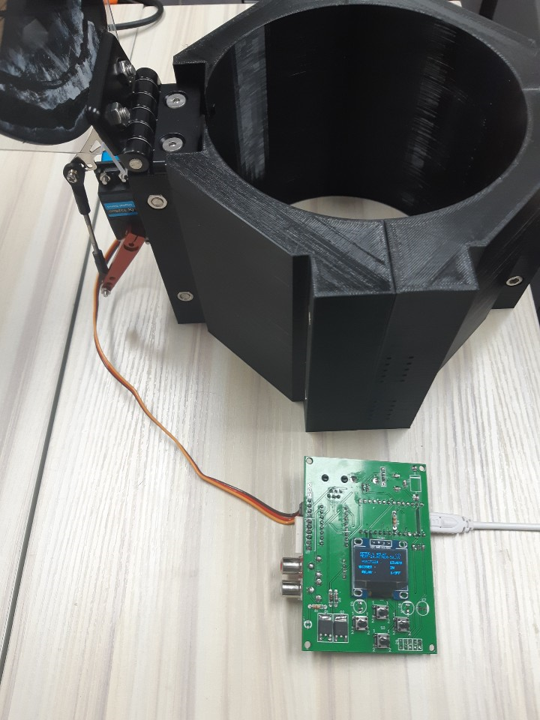
\includegraphics[height=7cm]{mask_status1}
			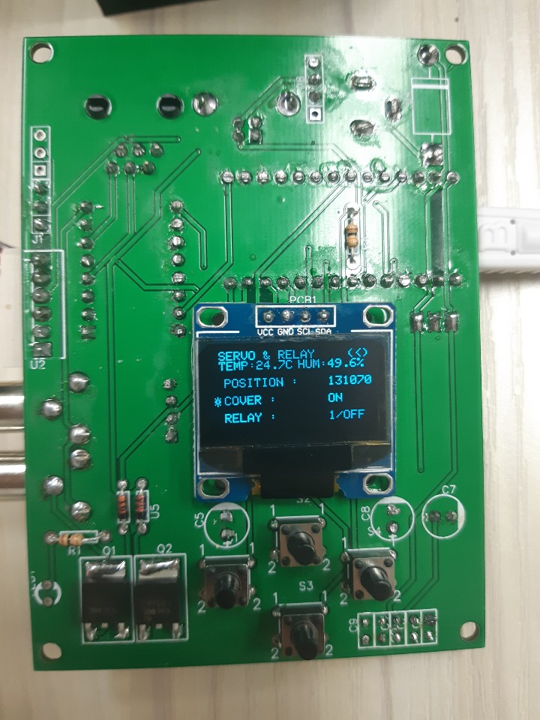
\includegraphics[height=7cm]{mask_status2} 
		};
		\draw (0.35, 0.3) node {(a)};
		\draw (5.7, 0.3) node {(b)};
		\end{tikzpicture}
	\end{center}
	\caption{(a) 개선된 모터포커서를 이용하여 제어한 덮개 (b) 이 때 개선된 모터포커서에 출력되는 마스크의 상태. 화면 아래의 버튼들을 이용해 상태를 제어할 수 있으며, 제어상태를 확인할 수 있다.}
\label{mask_status}


\end{figure}

\subsubsection{릴레이 스위치}

 릴레이 스위치는 6개의 핀으로 이루어져 있으며, 순서대로 +5v, GND, 1,2,3,4의 Relay이다. 때문에 각 핀들을 모두 연결시킨 뒤에 MCU를 이용하여 적절하게 제어할 수 있다. 각각의 기호는 P, Q, R, S이며, 상태만을 나타내기 때문에 서보모터 제어와 마찬가지로 오직 0과 1만을 입력받는다.
 
 
\newpage
\subsection{개선된 ASCOM 드라이버}


 기존의 모터포커서의 여러 기능들이 추가됨에 따라, 기존에 만들었던 ASCOM 호환 드라이버 또한 업데이트를 할 필요성이 있었다. 때문에 여러가지 기능들을 추가하여 기존의 GUI를 발전시켰으며, Fig\ref{maincontrol}은 발전시킨 ASCOM 드라이버의 GUI의 모습을 나타내었다.
 
 \begin{figure}[h]
	\begin{center}
		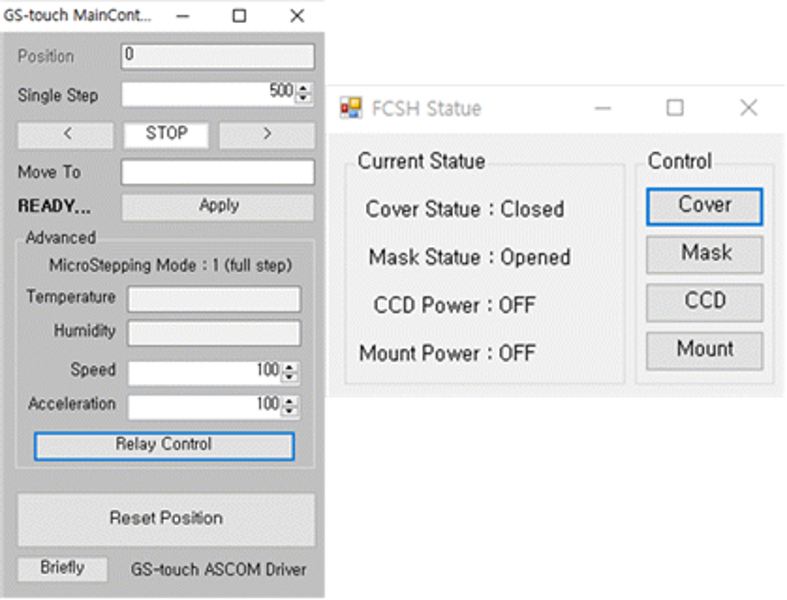
\includegraphics[width = 11cm]{maincontrol}
	\end{center}
	\caption{개선된 모터포커서 드라이버의 GUI 모습}
	\label{maincontrol}
\end{figure}

 기존의 모터포커서에서 추가된 기능인 덮개 제어기능, 열선 제어기능, Relay Control을 포함하고 있으며 각각의 Relay가 제어하는 기능들을 적었다.
